\section{EVALUATION }
\label{section:results}

\subsection{Simulation}
In this section, we try to simulate our sequence-based localization technique based on linear programming (LPSBL) with SBL method using MATLAB. 
In the simulation, we randomly generate a lot of smartphones in a $10m \times 10m$ area. 
Considering the impact of the uncertainty of node position and TOA detection, we add a certain amount of node location error and TOA measure error in all the simulations.
All the statistics are running more than 100 times for high confidence, and reported by RMSE figure. Table 1 illustrates the default simulation setup parameters.

\begin{table} \normalsize
\caption {\textbf{Default configuration parameter}} %title of the table
\centering % centering table
    \begin{tabular}{|c|c|}
        \hline
Parameter & Description \\
 \hline
Field Area & 10m $\times$ 10m \\
\hline
Number of Anchors & 50 (Default) \\
 \hline
Node Location Error 	 & 0.10m (Default) \\
 \hline
TOA Detection Error 	 & 0.10ms (Default) \\
 \hline
Random-Seed Loop	 & 500 times (Default) \\
 \hline
Error Statistics	 &  RMSE \\
        \hline
    \end{tabular}
\end{table}



The results of simulation evaluation are as following:


\textbf{1) Impact of the number of anchors:}
 In this experiment, we investigate the localization error and number of anchors with a different number of anchors from 10 to 40 in steps of 2. 
 We run the simulation with the TOA error is 0.1ms, and other simulation parameters are default. 
 Since the two localization methods being compared are aiming to locate the target by processing the anchors, 
 but the SBL method can cause a big error, while the LPSBL method is aiming to avoid the appearance and get better result. 
 We can speculate that with more anchors, the whole area will be divided into smaller parts, 
 thus more accurate localization estimation should be achieved in the LPSBL method. 
Fig. \ref{fig4} confirms our expectation. As shown in Fig. \ref{fig4}, with the number of anchors increases, localization error for both  methods are down slowly. 
Fig. \ref{fig4} also shows that the localization error caused by the LPSBL method is smaller than the SBL method when the number of anchor node is less.
  \begin{figure}[htb]
            \setlength{\abovecaptionskip}{0pt}
           % \centering
			 \vspace{-15mm}
           		 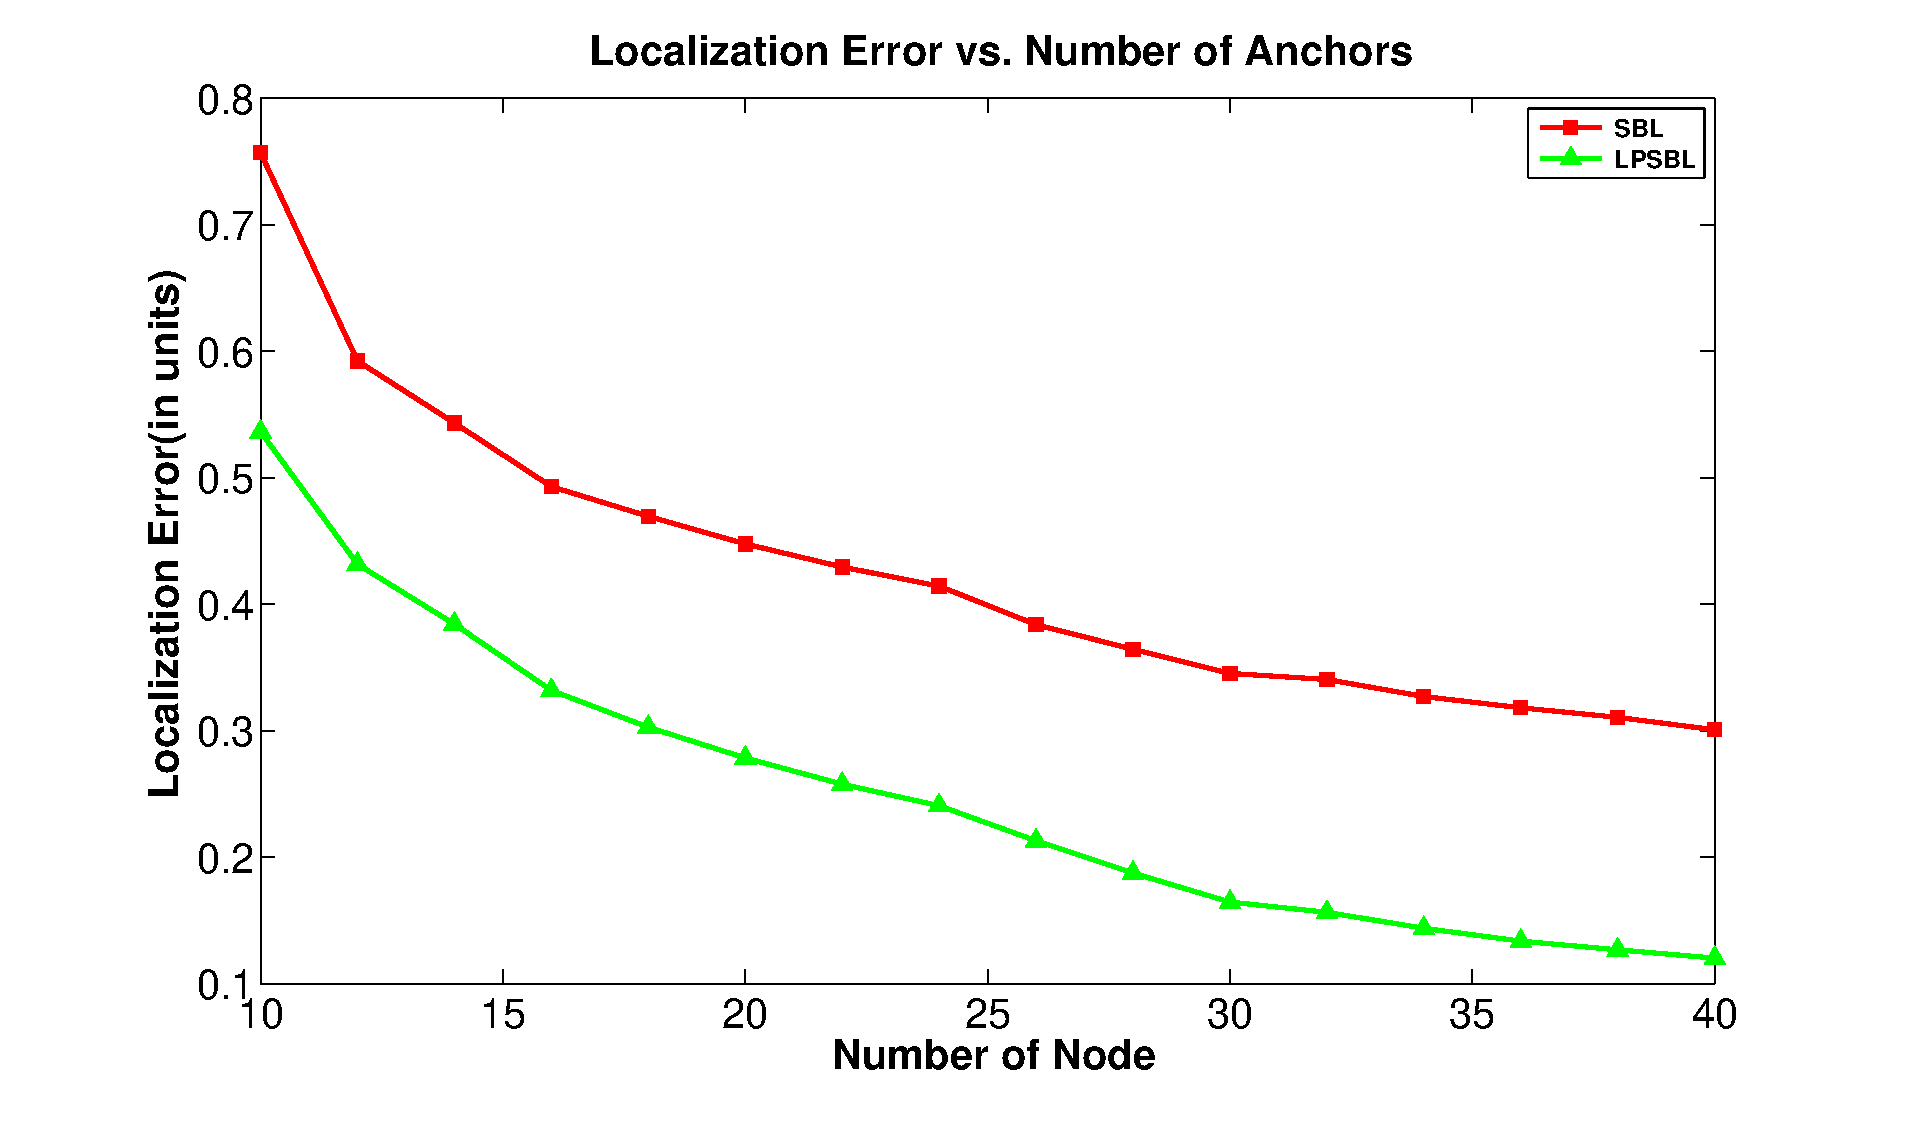
\includegraphics[height=5.0cm,width=7.0cm]{image/fig4.eps}
            \vspace{15mm}
            \caption{Localization Error vs. Number of Anchors}
             \vspace{-7mm}
             \label{fig4}
        \end{figure}	
		
\textbf{2) Impact of the location error:}
 In this experiment, we compare the two methods for different location errors of anchors. 
 In Fig. \ref{fig5}, we choose the location error with the range from 0 to 0.4m in step of 0.02m for the two methods. 
 Fig. \ref{fig5} indicates the location error of anchors has an effect on the positioning results. 
 The proposed LPSBL method are more accurate than the SBL method. 
 For the SBL method, the positioning error changes obviously as location error increases in Fig. \ref{fig5}. 
 However, as demonstrated in Fig. \ref{fig5}, the positioning error of LPSBL varies little, which demonstrates the LPSBL method is the most robust to the node location error.
  \begin{figure}[htb]
          %  \centering
		   \vspace{-25mm}
			 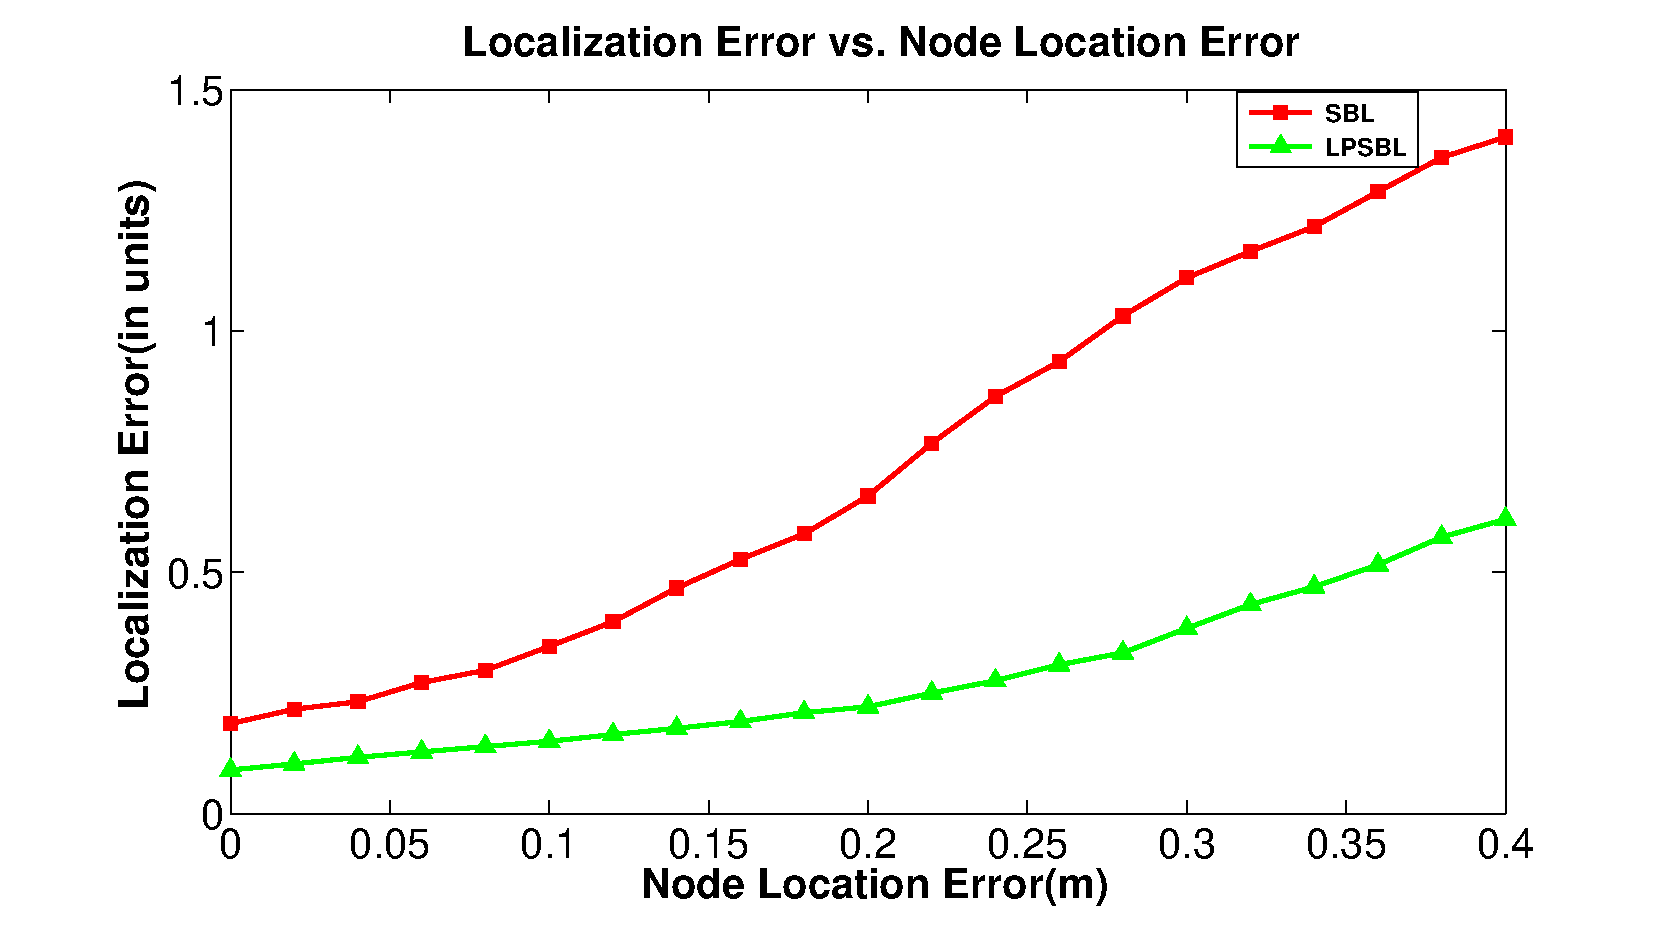
\includegraphics[height=5.0cm,width=7.0cm]{image/fig5.eps}
            \vspace{25mm}
            \caption{Localization Error vs. Node Location Error}
             \vspace{-5mm}
             \label{fig5}
        \end{figure}

\textbf{3) Impact of the TOA measurement error:}
In this experiment, we perform the impact of the TOA error of anchors for the two methods being compared with the range from 0 to 2ms in steps of 0.1ms. 
Other simulation parameters keep default. 
We can guess that the TOA measurement error may influence the localization accuracy. 
Fig. \ref{fig6} confirms it. As it is shown in Fig. \ref{fig6}, the localization error of the  two methods is increasing as the TOA error growth. 
Thus, we can determine the speculation that the error of TOA measurement can influence the localization accuracy is true. 
Also, the LPSBL method has a better result than the SBL method. 
%The Robust LPSBL method get the best experimental result. 
It is shown in Fig. \ref{fig6}, the localization error of our LPSBL method is stable no matter which degree the TOA error is, which means that the LPSBL method can localize the target node with little error when TOA error is not too big.
  \begin{figure}[htb]       
           % \centering
			\vspace{-15mm}
            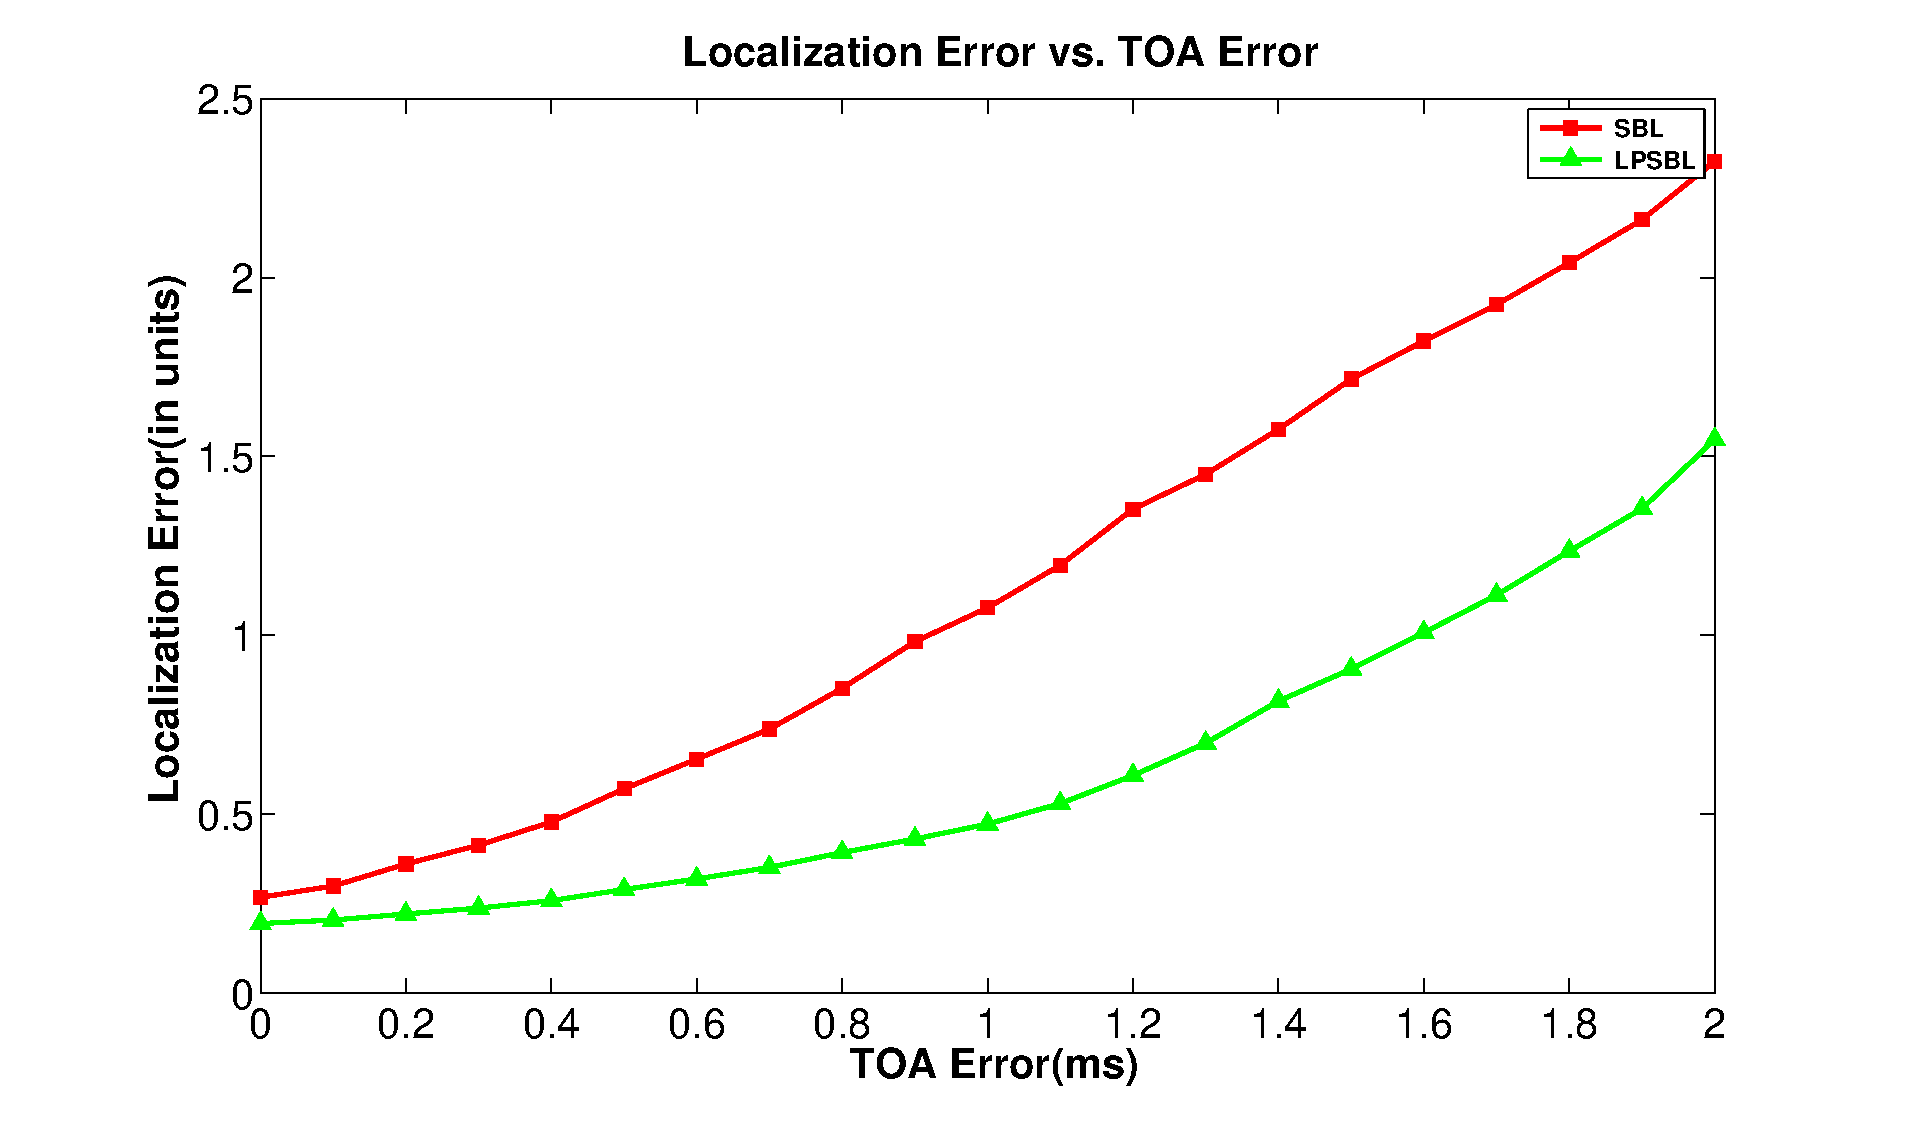
\includegraphics[height=5.0cm,width=7.0cm]{image/fig6.eps}
           \vspace{15mm}
            \caption{Localization Error vs. TOA Error}
             \vspace{-5mm}
             \label{fig6}
        \end{figure}
 \textbf{Summary:} From the above simulations, considering the different factors, including the number of anchors, the node location error and TOA measurement error of the anchors, we can get the following conclusions:

 (1) With increasing number of the number of anchors, localization errors decrease for both methods, and LPSBL has better localization performance;

 (2) The error of node location can impact the localization error, the proposed LPSBL method is more robust to the error of node location than SBL method;
 
 (3) The TOA measurement error has a major impact on the localization accuracy, and the proposed LPSBL method can achieve better localization performance.



\subsection{Emulation}


In this section, we report system implementation of our design based on smartphones.
we use 30 Samsung smartphones as anchors and connect them through CISCO CVR328W-K9-CN wireless router. 
TPSN protocol is adapted in the proposed LPSBL system to realize time synchronization.
The 30 smartphones are deployed in a size of 16m$\times$10m space and there just one target during an experiment.
In the experiment, smartphones are random deployed in the space, and 100 times localization results are showed in Fig.~\ref{fig7}. 
In the figure, blue squares stand for anchor
nodes, red circle squares are the real position of acoustic sources, and black dot are the estimated location by LPSBL. 
An arrow origins from the estimated location of each acoustic source and points to its real position. 
As the results showed in Fig.\ref{fig7}, most of estimated locations are close to the ground truth and the errors between them are very small,
which means that LPSBL can effectively localize the acoustic source with good robustness.
  \begin{figure}[htb]
              %    \centering
			    \vspace{-12mm}
            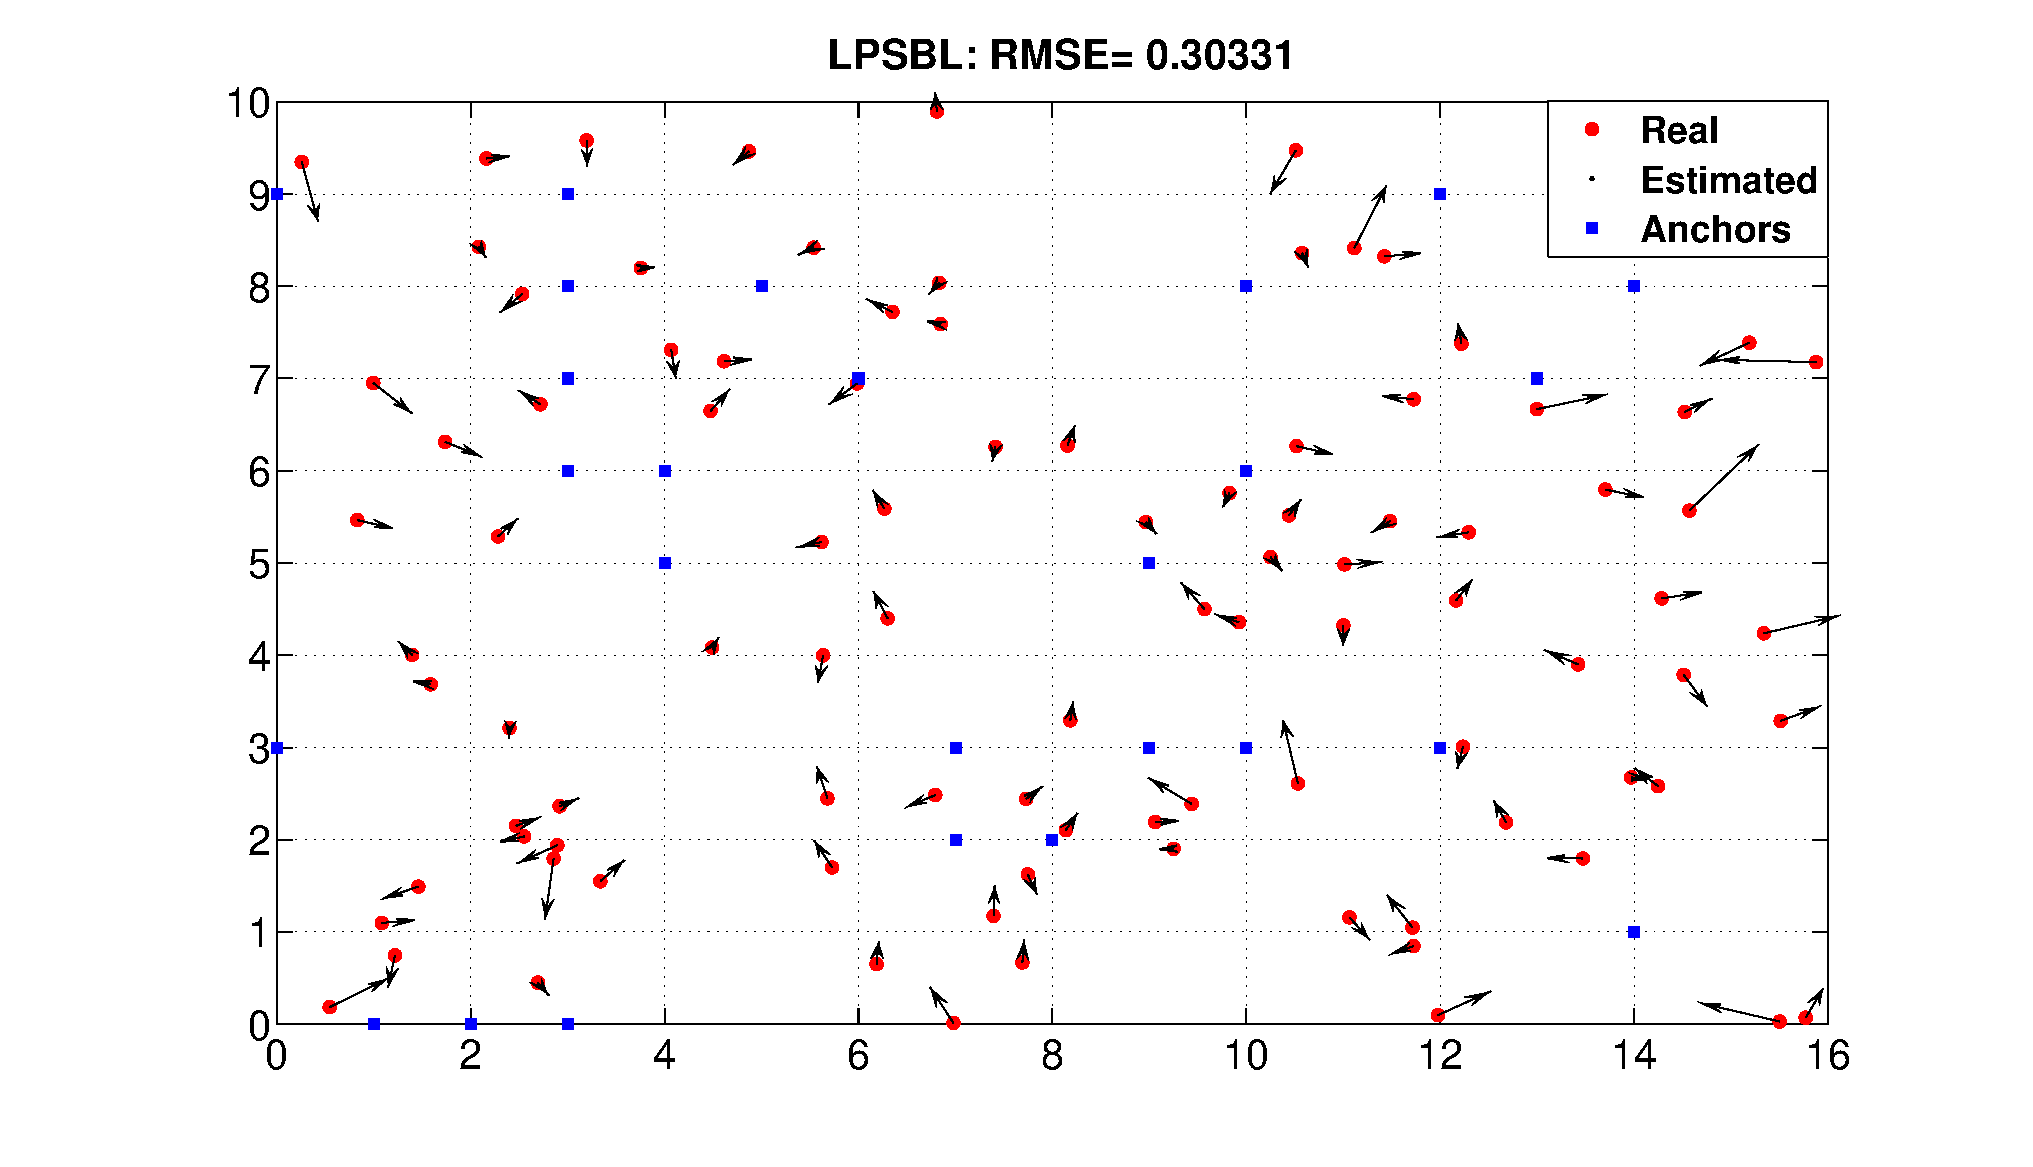
\includegraphics[height=5.0cm,width=7.0cm]{image/fig7.eps}
            \vspace{12mm}
            \caption{Test-bed localization result of the proposed LPSBL}
             \vspace{-5mm}
             \label{fig7}
        \end{figure}
